% !TEX root = ./multilinear.tex
\section{Preliminaries}
\label{sec:prelim}

\subsection{Problem Formulation and Notation}
We will focus primarily on the following two classes of problems in this paper; our
approach can be extended more broadly.

\noindent
%\textbf{Finding Paths and Trees}
\subsubsection{Finding Paths and Trees}
Given a graph $G=(V, E)$ with $n=|V|$, $m=|E|$, and a subgraph $H=(V_H, E_H)$, with $k=|V_H|$, the basic subgraph isomorphism problem involves finding a mapping $f:V_H\rightarrow V$,
such that $(i, j)\in E_H$ if and only if $(f(i), f(j))\in E$.

\begin{problem} ($k$-Tree)
\label{prob:trees}
Given a weighted graph $G=(V, E)$ with a weight vector $\mathbf{w}$, and a tree
denoted by $H=(V^H, E^H)$ with $|V^H|=k$, the objective is to determine if there exists
an embedding of $H$ in $G$.
\end{problem}

Other common variants of this problem are: (1) counting all embeddings, and (2) finding a maximum
weight embedding in a weighted version of the graph; our approach can be extended to all
these variants.


\noindent
%\textbf{Anomaly Detection Using Graph Scan Statistics}
\subsubsection{Anomaly Detection Using Graph Scan Statistics}
We use the notation of \cite{cadena:sdm17} here. We assume each node $v\in V$ has two associated values,
which vary with time (we will not show the time, to avoid complicating the notation):
(1) a \emph{baseline count}, $b(v)$, which indicates the count that we
expect to see at the node $v$---e.g., the number of people in a county corresponding to node $v$---and
(2) an \emph{event count} or \emph{weight}, $w(v)$, which indicates how many occurrences of an event
of interest are seen at the node---e.g., the number of cases of a disease in a county.

Graph scan statistics are among the most commonly used methods for detecting anomalies or ``hotspots" in
networked data \cite{Speakman-14,leiserson2015pan, hansen2016finding, neil2013scan, chen2014non}.
Informally, this approach formalizes anomaly detection as a hypothesis testing problem.
Under the null hypothesis $H_0$, it is \emph{business as usual}, and the event counts for all nodes are generated proportionally to their baseline counts. Under the alternative hypothesis $H_1(S)$, counts of a majority of
the vertices are generated (again) with rate proportional to the baseline counts, but there exists a small connected subset
$S \subseteq V$ of vertices for which the counts are generated at a higher rate than expected.
Then, the goal is to find a set of vertices $S$ that maximizes an appropriate scan statistic function $F(S)$, typically a log-likelihood ratio that compares event counts to baseline counts. We define a scan statistic in terms of the event and baseline counts of a node set:
$$
F(S) = F(W(S), B(S), \mathbf{\theta}),
$$
where $W(S) = \sum_{v \in S} w(v)$ is the total event count or \emph{weight} of $S$, $B(S) = \sum_{v \in S} b(v)$ is the baseline count of the set, and $\theta$ represents possible additional arguments to $F$.

The graph anomaly detection problem can be posed as the following constrained optimization problem.

\begin{problem}
\label{prob:macs}
Given a graph $G=(V, E)$, a scan statistic $F(\cdot)$, the associated counts for vertices---$\mathbf{w}$ and $\mathbf{b}$---and a parameter $k$, find a connected subset $S\subseteq V$ that maximizes $F(S) = F(W(S), B(S), \theta)$ with $B(S) \leq k$.
\end{problem}

\noindent
\textbf{Our approach.} Problems \ref{prob:trees} and \ref{prob:macs} are seemingly very different,
and are computationally very challenging. Problem \ref{prob:macs}
has been shown to be NP-hard in general \cite{cadena:sdm17}. Finding paths of length at least $k$
is NP-hard when $k$ is large. We will focus on the setting where $k$ is small, e.g., $O(\log{n})$.
The only prior approach that has given algorithms with rigorous bounds for these two problems
involves the use of the technique called \emph{color coding} (\cite{alon2008biomolecular, huffner2008algorithm,
alon1995color} for Problem \ref{prob:trees} and \cite{cadena:sdm17} for Problem \ref{prob:macs}).
However, color coding has a significant memory overhead, and we propose a new approach
based on an algebraic technique that involves detecting multilinear terms in multivariate polynomials.
We first discuss the basic theoretical concepts needed for this approach, and then the seminal
algorithm of \cite{DBLP:journals/talg/KoutisW16, williams2009finding} for multilinear detection.
Our approach involves two steps:
\begin{itemize}
\item
We develop an MPI-based parallel algorithm for multilinear detection of any multivariate
polynomial, represented as a directed acyclic graph (DAG) (Section \ref{sec:proposed}).
\item
We show that both our problems can be reduced to multilinear detection for suitably defined
polynomials, and thus can be solved in parallel. The parallel algorithm in Section \ref{sec:proposed}
is described for any multivariate polynomial, represented as a DAG, and
serves as an abstraction.% for describing both algorithms. 
We discuss how the specific
polynomials (and DAGs) are constructed for our problems.
\end{itemize}


\subsection{The Multilinear Detection Problem}
Let $X = x_1, \ldots,x_n$ be a set of variables, and let $P(X)$ be a polynomial, which is a sum 
of monomials on $X$. We will denote $P(X)=\sum_S \Pi_{i\in S} x_i$ as a monomial, where
the sum is over multisets $S$.  An example of a polynomial on six variables is 
$P(x_1,x_2,x_3,x_4, x_5, x_6) = x_1^2x_2 + x_2x_3x_4 + x_3x_4x_5 + x_5x_6$. 
A monomial is called \emph{multilinear} or \emph{square-free} if all its variables 
have exponent 1, and its \emph{degree} is the sum of the exponents of all its variables. 
For instance, in the example above, $x_2x_3x_4$, $x_3x_4x_5$, and $x_5x_6$ are multilinear monomials, but $x_1^2x_2$ is not multilinear. 
Given variables $X = x_1, \ldots ,x_n$ and a polynomial $P(X)$, the goal in 
the $k$-Multilinear Detection (\textsc{$k$-MLD}) problem
is to decide whether or not $P(X)$ has a multilinear monomial of degree exactly $k$. 


We note that the polynomial $P(X)$ may have an arbitrary number of terms---i.e., exponential on the size of $n$---therefore, the problem is not as simple as writing the polynomial explicitely and checking each term. Rather, we assume that $P(X)$ is given succintly in a recursive form, and the ``yes"/``no" decision has to be made without unrolling this recursion.
Figure \ref{fig:dag} illustrates a circuit representation of the polynomial $P(\cdot)$ above.
In general, we also have a weight $w_S$ for each multinomial $\Pi_{i\in S} x_i$ corresponding
to each term in the polynomial $P(\cdot)$. Our focus in this paper will be the following problem.

\begin{figure}[h]
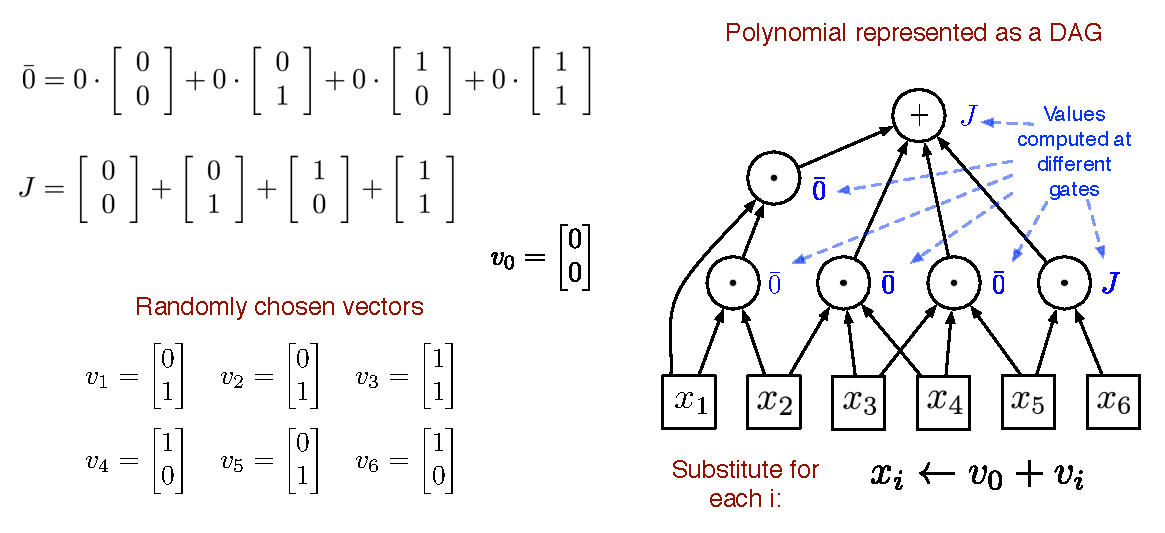
\includegraphics[width=0.5\textwidth]{img/dag3_fixed.pdf}
\caption{
\small
The polynomial $P(x_1,x_2,x_3,x_4, x_5, x_6) = x_1^2x_2 + x_2x_3x_4 + x_3x_4x_5 + x_5x_6$
represented as a circuit with multiplication ($\cdot$) and addition ($+$) gates, which is a DAG. 
Each variable $x_i$ is assigned the element $v_0+v_i\in\mathbb{Z}_2[\mathbb{Z}_2^2]$,
for randomly chosen $v_i\in \mathbb{Z}_2^2$. The computations at each gate
are in the group algebra, and are shown in blue. The circuit evaluates to the element $J$.
\vspace{-0.2in}
}
\label{fig:dag}
\end{figure}

\begin{problem} (\textsc{$k$-MLD} problem)
Given a polynomial $P(\cdot)$ represented by a DAG $G=(V, E)$, in which each monomial
has degree at most $k$, with a weight $w_S$ for
each monomial corresponding to the multiset $S$ in $P(\cdot)$, determine:
(1) if $P(\cdot)$ has a multilinear term, and 
(2) the maximum weight of any multilinear term, if one exists.
\end{problem}


\subsection{Group Algebras}
\label{sec:grpalgebra}
We discuss some notation from group algebras that is crucial for the paper. 
Let $\mathbb{Z}_2^k$ be the group formed by all the $k$-dimensional binary vectors, and define the group multiplication operation as entry-wise XOR. For example, $\mathbb{Z}_2^2$ consists of the vectors $v_0 = (0, 0), v_1 = (0, 1), v_2 = (1, 0), v_3 = (1, 1)$. We note that $v_0$ is the multiplicative identity of the group, and each element is its own multiplicative inverse: $v_i \cdot v_i = v_0$. Now, we define a group algebra $\mathbb{Z}_2[\mathbb{Z}_2^k]$. Each element in the group algebra is a sum of elements from $\mathbb{Z}_2^k$ with coefficients from $\mathbb{Z}_2$ (i.e., either 1 or 0):
$
\sum_{v\in \mathbb{Z}_2^k} a_v v,
$
where $a_v \in \{0,1\}$. The addition operator of the group algebra is
{\scriptsize
$$
\sum_{v\in \mathbb{Z}_2^k} a_v v + \sum_{v\in \mathbb{Z}_2^k} b_v v = \sum_{v\in \mathbb{Z}_2^k} (a_v + b_v) v,
$$}
where the addition of the coefficients is modulo 2, and the multiplication is defined as
{\scriptsize
$$
\left(\sum_{v\in \mathbb{Z}_2^k} a_v v\right)\left(\sum_{u\in \mathbb{Z}_2^k} b_u u\right) = \sum_{v\in \mathbb{Z}_2^k} (a_v \cdot b_u) (v\cdot u).
$$}


\begin{mdframed}
\scriptsize{
\noindent
\textbf{Example.} For $k=2$, the group algebra $\mathbb{Z}_2[\mathbb{Z}_2^k]$ has
$2^{2^2}=16$ elements, such as
\[
x_1=
0\cdot
\begin{bmatrix}
0\\
0
\end{bmatrix}
+ 1\cdot
\begin{bmatrix}
0\\
1
\end{bmatrix}
+
1\cdot
\begin{bmatrix}
1\\
0
\end{bmatrix}
+ 0\cdot
\begin{bmatrix}
1\\
1
\end{bmatrix}
, \mbox{ which we also write as }
\begin{bmatrix}
0\\
1
\end{bmatrix}
+
\begin{bmatrix}
1\\
0
\end{bmatrix}
\]


\[
x_2 =
\begin{bmatrix}
0\\
0
\end{bmatrix}
+
\begin{bmatrix}
1\\
0
\end{bmatrix}
\]

We have 
\[
x_1 + x_2 = 
\begin{bmatrix}
0\\
0
\end{bmatrix}
+
\begin{bmatrix}
0\\
1
\end{bmatrix}
+ 2
\begin{bmatrix}
1\\
0
\end{bmatrix}
=
\begin{bmatrix}
0\\
0
\end{bmatrix}
+
\begin{bmatrix}
0\\
1
\end{bmatrix}
\]

\[
x_1x_2 = 
\left(
\begin{bmatrix}
0\\
1
\end{bmatrix}
+ 
\begin{bmatrix}
1\\
0
\end{bmatrix}
\right)\cdot 
\left(
\begin{bmatrix}
0\\
0
\end{bmatrix}
+
\begin{bmatrix}
1\\
0
\end{bmatrix}
\right) =
\begin{bmatrix}
0\\
0
\end{bmatrix}
+
\begin{bmatrix}
0\\
1
\end{bmatrix}
+
\begin{bmatrix}
1\\
0
\end{bmatrix}
+
\begin{bmatrix}
1\\
1
\end{bmatrix}
\]
It is easy to check that
\[
x_1^2x_2 = 
0\cdot
\begin{bmatrix}
0\\
0
\end{bmatrix}
+ 0\cdot
\begin{bmatrix}
0\\
1
\end{bmatrix}
+ 0\cdot
\begin{bmatrix}
1\\
0
\end{bmatrix}
+ 0\cdot
\begin{bmatrix}
1\\
1
\end{bmatrix}
= \mathbf{\bar{0}} \text{ (additive identify)}
\]
}
\end{mdframed}

\subsection{Sequential algorithm for Multilinear Detection} 
\label{sec:seq}
We briefly discuss the algorithm of Koutis \cite{koutis:icalp08}, which forms the basis of our paper. An important property is that for any $v_i \in \mathbb{Z}_2^k$, the square of the term $(v_0 + v_i) \in \mathbb{Z}_2[\mathbb{Z}_2^k]$ evaluates to 0:
{\small
$$
(v_0 + v_i)^2 = v_0^2 + 2(v_0\cdot v_i) + v_i^2 = v_0 + (0\mod 2)v_i + v_0 = 2v_0 = 0.
$$}

The main idea in the algorithm of \cite{koutis:icalp08} is that, if we evaluate a polynomial 
over the ``right" algebra, monomials that have square terms evaluate to 0, and the remaining terms,
which are multilinear, do not cancel out, with some probability.
Then, a polynomial $P(X)$ has a $k$ multilinear term if $P(X) \neq 0$. 

We can show that, if we choose a $v_i \in \mathbb{Z}_2^k$ uniformly at random and set $x_i = v_0 + v_i$, then a multilinear monomial does \textbf{not} evaluate to $\bar 0$ with high probability, whereas a monomial with squares is always $\bar 0$ (as in the box above).
The algorithm was later refined in \cite{williams2009finding} by evaluating the polynomial over the group algebra $GF(2^{3 + \log_2k})[\mathbb{Z}_2^k]$, where $GF(p)$ is the finite field of order $p$ \cite{mullen2007finite}. A polynomial $P(x_1,\ldots,x_n)$ with variables from $GF(2^{3 + \log_2k})[\mathbb{Z}_2^k]$ can be evaluated in time $O(2^k poly(n))$ and space $O(kpoly(n))$, resulting in Theorem \ref{theorem:kmld}.

\begin{theorem}[Koutis \cite{koutis:icalp08} and Williams \cite{williams2009finding}]
\label{theorem:kmld}
There exists an algorithm that, given an instance $P(x_1,\ldots,x_n)$ of the \textsc{$k$-MLD} problem, correctly returns ``no" if $P(X)$ does not contain a $k$ multilinear term. Otherwise, if $P(X)$ has a $k$ multilinear term, it returns ``yes" with probability at least 1/5. 
The algorithm has time complexity $O(2^k poly(n))$ and space complexity $O(2^k poly(n))$.
\end{theorem}

At a high level, the algorithm of \cite{koutis:icalp08} involves the following steps.
\begin{enumerate}
\item For each variable $x_i$, sample a vector $v_i$ uniformly at random from $\mathbb{Z}_2^k$ and assign $x_i = (v_0 + v_i) \in \mathbb{Z}_2[\mathbb{Z}_2^k]$.
\item Evaluate the polynomial $P(x_1,\ldots,x_n)$ on this random assignment.
\item If $P(x_1,\ldots,x_n) \neq \bar{0}$ return ``yes"; otherwise, return ``no",
where $\bar{0}$ is the additive identity of the group algebra.
\end{enumerate}

%For the case when a multilinear monomial appears an odd number of times in $P(X)$, Koutis proposed a randomized algorithm that runs in $O(2^k poly(n))$ time and returns an affirmative answer with probability at least $1/4$ \cite{koutis:icalp08}. This algorithm was later extended by Williams \cite{williams2009finding} to allow even repetitions.

%It has been shown that many parameterized graph problems reduce to \textsc{$k$-MLD} \cite{koutis:icalp08,williams2009finding,guillemot2013finding,koutis2012constrained} by efficiently encoding subgraphs of interests as monomials. For example, in the $k$-path problem\footnote{In the $k$-path problem, we are given an unweighted graph $G(V,E)$, and the goal is to decide whether or not there is a simple path containing exactly $k$ nodes in $G$.}, it is possible to recursively construct a polynomial in which each term represents a walk of length $k$, and only multilinear terms correspond to simple paths. Our algorithms in Section \ref{sec:proposed} are based on this methodology: we encode subgraphs of a given size and weight as polynomials, and only connected subgraphs of size at most $k$ where all the nodes are different are multilinear terms.



%Now, we define a group algebra $\mathbb{Z}_2[\mathbb{Z}_2^k]$. Each element in the group algebra is a sum of elements from $\mathbb{Z}_2^k$ with coefficients from $\mathbb{Z}_2$ (i.e., either 1 or 0):
%$$
%\sum_{v\in \mathbb{Z}_2^k} a_v v,
%$$
%where $a_v \in \{0,1\}$. Such element may also be interpreted as a subset of $\mathbb{Z}_2^k$---because of the binary coefficients. The addition operator of the group algebra is
%$$
%\sum_{v\in \mathbb{Z}_2^k} a_v v + \sum_{v\in \mathbb{Z}_2^k} b_v v = \sum_{v\in \mathbb{Z}_2^k} (a_v + b_v) v,
%$$
%where the addition of the coefficients is modulo 2. The multiplication is defined as
%$$
%\left(\sum_{v\in \mathbb{Z}_2^k} a_v v\right)\left(\sum_{u\in \mathbb{Z}_2^k} b_u u\right) = \sum_{v\in \mathbb{Z}_2^k} (a_v \cdot b_u) (v\cdot u).
%$$
%

%The key insight in \cite{koutis:icalp08} is that, for any $v_i \in \mathbb{Z}_2^k$,
%{\small
%$$
%(v_0 + v_i)^2 = v_0^2 + 2(v_0\cdot v_i) + v_i^2 = v_0 + (0\mod 2)v_i + v_0 = 2v_0 = 0 \mod 2.
%$$}
%If we are given a polynomial $P(X)$, and we assign uniformly at random an element $(v_0 + v_i)$ from $\mathbb{Z}_2[\mathbb{Z}_2^k]$ to each $x_i$ variable, then, any monomial with a square term will evaluate to 0. This is called the \emph{annihilation} property. The second key idea is that, under this random assignment, a multilinear monomial does not evaluate to 0 with high probability. This is called the \emph{survival} property. Finally, Koutis shows that a polynomial $P(x_1,\ldots,x_n)$, where the variables are elements from $\mathbb{Z}_2[\mathbb{Z}_2^k]$, can be evaluated in time $O(2^k poly(n))$ and space $O(kpoly(n))$.

%Because of the choice of binary coefficients in the group algebra and the modulo 2 addition operation, any monomial that appears an even number of times in $P(X)$ will evaluate to $0$. In \cite{williams2009finding}, Williams proposes working with the group algebra $GF(2^{3 + \log_2k})[\mathbb{Z}_2^k]$, where $GF(p)$ is the finite field of order $p$ \cite{mullen2007finite}. By using this group algebra, it is unlikely that multilinear monomials evaluate to 0 merely due to repetition, and, at the same time, the annihilation property of \cite{koutis:icalp08} is preserved. We have the following theorem.

\comment{add sequential algorithm in supplementary and refer to it here}

\subsection{Implementing The Sequential Algorithm Using a Matrix Representation
of $\mathbb{Z}_2[\mathbb{Z}_2^k]$}

Theorem \ref{theorem:kmld} performs operations in the group algebra $\mathbb{Z}_2[\mathbb{Z}_2^k]$,
which takes $O(2^k poly(n))$ space. Koutis \cite{koutis:icalp08} showed that, in fact, the space
complexity can be reduced to $O(k poly(n))$ by using the idea of matrix representations.
%We describe this approach here and then the sequential algorithm \maxwt{} for $k$-MLD. We will develop the parallel version of this algorithm in Section \ref{sec:proposed}.
We use the notation from \cite{koutis:icalp08} and describe it here for completeness.
Let $\rho:\mathbb{Z}_2^k\rightarrow M^{2^k\times 2^k}$ be a matrix representation of
$\mathbb{Z}_2^k$ satisfying $\rho(uv)=\rho(u)\rho(v)$ for all $u, v\in \mathbb{Z}_2^k$.
For $k=1$, the map $\rho:\mathbb{Z}_2\rightarrow M^{2\times 2}$ is defined as
\[
\rho(0) = 
\begin{bmatrix}
1 & 0\\
0 & 1
\end{bmatrix}
\mbox{ and }
\rho(1) = 
\begin{bmatrix}
0 & 1\\
1 & 0
\end{bmatrix}
\]

In general, $\rho(\mathbb{Z}_2^k)$ can be defined recursively. We will use a
simultaneous diagonalization, which allows $\rho(v)$ to be represented as
$\rho(v) = U^{-1}\Lambda_v U$, for each $v\in \mathbb{Z}_2^k$, where $\Lambda_v$ is
a diagonal matrix with its $t$th element equal to $(-1)^{v^T t_{bin}}$,
where $t_{\text{bin}}$ is the $k$-bit binary representation of $t$.
Since the algorithm substitutes $v_0+v_i$ for each variable $x_i$ (as shown in
Figure \ref{fig:dag}), the $t$th element of the diagonal element in the corresponding
representation for $\rho(v_0+v)$ is $1+(-1)^{v^T t_{bin}}$.

%We now describe the sequential algorithm \maxwt{} for the $k$-MLD problem. We are given a graph $G(V,E)$ and a parameter $k$, which together constitute an instance of $k$-MLD. 

